\documentclass[compress,11pt]{beamer}

% language and encodings
\usepackage[english]{babel}
\usepackage[utf8]{inputenc}
\usepackage[T1]{fontenc}
\usepackage{comment}
\usepackage{media9}
\usepackage{graphicx}
\usepackage{multimedia}
\usepackage{multirow}



% TikZ
\usepackage{tikz}
\usetikzlibrary{mindmap,trees}
\tikzset{every node/.append style={scale=0.6}}
\usepackage{smartdiagram}

\smartdiagramset{
	planet size=3cm,
	planet text width=2.5cm,
	planet font=\footnotesize,
	satellite size=2cm, 
	satellite text width=2.5cm,
	satellite font=\scriptsize,
	distance planet-text=0,
	%distance satellite-text=0,
	distance planet-satellite=3.5cm,
	/tikz/connection planet satellite/.append style={>-}
}

\tikzset{priority arrow/.append style={rotate=180,anchor=0,xshift=30,}}% reversing arrow

% Beamer theme - options:
% - navigationDotsLocation: specify location of the dots in the headline
%   - near: display the dots near the section names (default)
%   - below: display the dots below the section names
% - titlePageSpacing: vertical spacing between items on title page (default: 1.5em)
% - titlePageNumberOfAuthors: influence size and location of authors on title page
%   - few (default): use larger font size, display authors on the left
%   - many: use smaller font size, display authors on the right
% - thanksPageBigGraphicsScale: scale for the big graphics on the thanks page (default: 1)
% - titlePageUniversityLogo: location of university logo file on the title page
%   (default: ../gfx/logos/logo_us_white)
% - titlePageInstituteLogo: location of institute logo file on the title page
%   (default: ../gfx/logos/logo_ipvs)
% - titlePageDepartmentLogo: location of department logo file on the title page
%   (default: ../gfx/logos/logo_sgs)
% - titlePageBigLogo: location of big logo file on the title page
%   (default: ../gfx/logos/logo_simtech)
% - thanksPageBigGraphics: location of the big graphics on the thanks page
%   (default: ../gfx/tikz/gfx_title)
% - thanksPageInstituteLogo: location of institute logo file on the thanks page
%   (default: ../gfx/logos/logo_ipvs)
% - thanksPageDepartmentLogo: location of department logo file on the thanks page
%   (default: ../gfx/logos/logo_sgs)
% - thanksPageBigLogo: location of big logo file on the thanks page
%   (default: ../gfx/logos/logo_simtech)
\usetheme[
    thanksPageBigGraphics=../gfx/thanks,
    navigationDotsLocation=below,
    titlePageSpacing=0.6em,
    titlePageNumberOfAuthors=many,
]{Stuttgart}

% metadata
\title{Dynamic Load Carrying Capacity of a Robot Manipulator}
\subtitle{Metzingen, Germany}
\author{Mujiburrehman Gouri}

%\institute{Dipl.-Ing. Mavarick Ho \\ \vspace{0.2cm} \boldmath{ Hochschule Ravensburg-Weingarten} \\Prof. %Dr.-Ing. Lothar Berger \\Prof. Dr.-Ing. Raphael Ruf \\ \hspace{1.9cm}}

\institute{Prof. Dr.-Ing. Lothar Berger \\Prof. Dr.-Ing. Raphael Ruf \\ \boldmath{ Hochschule Ravensburg-Weingarten}\\ \vspace{0.2cm} Dipl.-Ing. Mavarick Ho \\Neura Robotics GmbH}

\date{\today}

\begin{document}
    \only<beamer>{\titleframe}


\begin{frame}{Overview}
    \tableofcontents
\end{frame}


\sectionframe{Introduction}

\section{Introduction}

\begin{frame}{Topic of investigation}
	\centering
	\scalebox{0.75}{
		\smartdiagram[constellation diagram]{Thesis topic,
			Parameter estimation, Kinematics \\ and \\ dynamics, Control scheme, Optimization}
	}
\end{frame}


\begin{frame}{What is DLCC}
	
	\vspace{1cm}
	\begin{minipage}[c][\textheight][t]{0.4\textwidth}
	\begin{figure}	
	\centering %width=1\textwidth
	\includegraphics[height=0.65\textheight, width=0.5\textheight]{gazebo_elfin5.jpg}
	\caption{LARA robot}
	\end{figure}
	\end{minipage}\hfill
	\begin{minipage}[c][\textheight][t]{0.6\textwidth}
	\begin{itemize}
		\item Maximum load robot can carry %provided that the motor torques do not exceed the limit
		\pause
		\item Joint torque decides the load carrying capacity of the robot
		\pause
		\item Dynamic load depends upon the end-effector motion
		\pause
		\item Payload capacity of LARA %is 5 kg 
		\pause
		\item Payload capacity changes for configuration close or away from robot
	\end{itemize}
	\end{minipage}

\end{frame}

\begin{frame}{What is the Goal}
	% maximum payload is not constant for all the configuration , dynamics should be considered
	\begin{itemize}
		\item Incorporate robot dynamics in trajectory planning
		\item $\tau = H{(q)}\ddot{q} + c(q, \dot{q}) + \tau_g(q)$
		\pause
		\item Robot motion can have joint jerks for payload exceeding limits
		\pause
		\item Minimizing the joint jerks reduces the wear and tear
		\pause
		\item Optimization problem is formulated
	\end{itemize}
	
\end{frame}


\begin{frame}{Problem statement}
		\smartdiagram[descriptive diagram]{
		{Mass,{To obtain the physical properties of the end-effector object}},
		{Optimize, {To optimize the trajectory for objective function}},
		{Control, To track the optimized trajectory},
		%{Label, Add labels on edges or arrows} \only<2->{one}
		}
\end{frame}
%TODO: put pause
\begin{frame}{Topic importance}
	
		\smartdiagram[descriptive diagram]{
		{Why mass?,{Precise motion in task space}},
		{Why Optimize?, {Trajectory with minimum energy and reduced wear-tear}},
		{Why Control?, Follow the desired trajectory},
		%{Label, Smooth and Jerk-free motion},
		}

\end{frame}



\begin{comment}
\sectionframe{Literature review}

\section{Literature review}

\begin{frame}{State of the art}

\centering	
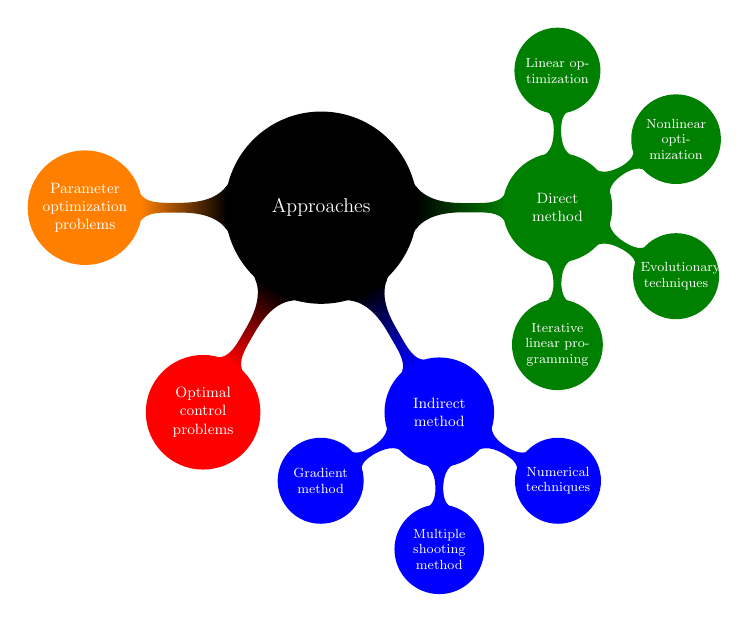
\begin{tikzpicture}[scale=0.6]
	\path[mindmap,concept color=black,text=white]
	node[concept] {Approaches}
	[clockwise from=0]
	child[concept color=green!50!black] {
		node[concept] {Direct method}
		[clockwise from=90]
		child { node[concept] {Linear optimization} }
		child { node[concept] {Nonlinear optimization} }
		child { node[concept] {Evolutionary techniques} }
		child { node[concept] {Iterative linear pro\-gramming} }
		%child { node[concept] {Stochastic technique} }
	}  
	child[concept color=blue] {
		node[concept] {Indirect method}
		[clockwise from=-30]
		child { node[concept] {Numerical techniques} }
		child { node[concept] {Multiple shooting method} }
		child {	node[concept] {Gradient method} }
	}
	child[concept color=red] { node[concept] {Optimal control problems} }
	child[concept color=orange] { 
	node[concept] {Parameter optimization problems}
	}
	;
\end{tikzpicture}
	
\end{frame}

\end{comment}

\sectionframe{Methodology}

\section{Methodology}

\begin{frame}{Inertial parameter estimation}
	
	A rigid body in space has following physical parameters,

    \begin{enumerate}
        \item
        Mass
        \pause

        \item
        Centre of mass
        \pause
        
         \item
        Moment of inertia
    \end{enumerate}

\end{frame}

% thesis page nr: 27
\begin{frame}{Mass estimation}
	
		\centering
		\scalebox{0.65}{
		\smartdiagram[priority descriptive diagram]{
		mass $= \dfrac{f}{gravity}$,
		Jacobian ($J$) Wrench ($f$) calculation $f = {J^{T}}^{-1} \delta \tau$,
		Change in torque $\delta \tau=\tau_1-\tau_2$ ,
		Joint torque with mass ($\tau_2$),
		Fix the joint position,
		Joint torque without mass ($\tau_1$)
			}
		}
\end{frame}

\begin{frame}{Centre of mass}
	
	    \centering
	    \scalebox{0.7}{
		\smartdiagram[priority descriptive diagram]{
		Least squares estimation for centre of mass ($r$) $r = {(F^T F)}^{-1} F^T M$,
		Avoid singular joint positions,
		Fill the data matrix with end-effector force ($F$) and torque($M$),
		Compute wrench ($f$) for different position
			}
		}
	
\end{frame}

\begin{frame}{Optimization}
	
	Optimization problem is formulated for trajectory planning
	
	
	\begin{enumerate}
		\item
		Cost functional formulation

		
	\end{enumerate}
	
\end{frame}

\begin{frame}{Cost functional}
	
	\vspace{1cm}
	\begin{minipage}[c][\textheight][t]{0.5\textwidth}
		\centering 
		\includegraphics[width=1\linewidth]{lara.pdf}
	\end{minipage}\hfill
	\begin{minipage}[c][\textheight][t]{0.5\textwidth}
		\begin{itemize}
			\item
			Robot motion from initial to goal position
			\pause
			\item 
			First objective is to track the desired trajectory
			\pause 
			\item 
			Secondary objective is to minimize the energy 
		\end{itemize}
	\end{minipage}
	
\end{frame}



\begin{frame}{First objective}
	
	\begin{itemize}
		\item
		Tracking of desired ($x_d$) and current position ($x_c$) as $x_d-x_c$
		\pause
		\item
		Nonlinear functions and inverse kinematics
		\pause 
		\item
		%We need to avoid nonlinear terms in cost functions 
		Tracking of velocity profile $\dot{x_d}-\dot{x_c}$
		\pause
		\item
		Using jacobian($J$), $\dot{x} = J_{(q)} \dot{q}$ 
		
	\end{itemize}
\end{frame}



\begin{frame}{Second objective}
	
	\begin{itemize}
		\item
		Kinetic energy of the robot, $K.E = \dfrac{1}{2} \dot{q}^T H \dot{q}$
		\pause
		\item
		Complex nonlinear terms and computation effort
		\pause
		\item 
		Joint acceleration for minimum energy, $K.E \approx \sum_{n=1}^{N}( \ddot{q}^{T}   \ddot{q} )$
		
	\end{itemize}
\end{frame}


\begin{frame}{Problem formulation}
	
		\centering
		\scalebox{0.52}{
		\smartdiagram[priority descriptive diagram]{
			Ensure joint torque limits,
			Solve the optimization,
			Equality constraint on desired position,			
			Inequality constraint on $\ddot{q}$ $\dot{q}$ and $q$, 
			Weight matrix to prioritize the cost function,
			Numerical gradient by finite-difference,
			Analytic gradient of the cost function,
			Cost functional $f(\boldmath{p})= w_{1}  \sum_{n=1}^{N}( \dot{x}_{d} - \dot{x}_{c} ) + w_{2}  \sum_{n=1}^{N}( \ddot{q}^{T}   \ddot{q} )$
			}
		}

\end{frame}

\begin{comment}

\begin{frame}{Control}
	
	Trajectory tracking after optimization.
	
	
	\begin{enumerate}
		\item
		Computed torque controller 
		
		
	\end{enumerate}
	
\end{frame}

\begin{frame}{Computed torque controller}
	
	\centering
	\scalebox{0.7}{
		\smartdiagram[priority descriptive diagram]{
			Follow the desired trajectory,
			Tune the PD gains,
			Calculate the dynamics of the robot,
			Control scheme,
			Setup torque controller with ROS
		}
	}
	
\end{frame}
\end{comment}



\sectionframe{Results}

\section{Results}

\begin{frame}{Inertial parameter estimation}
	
	\vspace{0.5cm}
	
	%\begin{minipage}[\textheight]{\textwidth}
	\begin{itemize}
		\item
		Friction is absent in robot simulation, $I_{F}=0$
		\pause
		
		\item
		Friction is present in robot hardware, $I_{F}\neq0$
		\pause
		
		\item
		$\tau = H{(q)}\ddot{q} + c(q, \dot{q}) + \tau_g(q) + \textcolor{red}{\bf{I_{F}}} $
		\pause
		
	\end{itemize}
	%\end{minipage}
	
	\vspace{0.5cm}
	
	\begin{minipage}[c][\textheight][t]{0.48\textwidth}
	\centering
	\begin{table}
		\centering
		\resizebox{\textwidth}{!}{%
			\begin{tabular}{|c|c|c|c|}
				\hline
				\multicolumn{2}{|c|}{\begin{tabular}[c]{@{}c@{}}Parameter\\ (unit)\end{tabular}} &
				\begin{tabular}[c]{@{}c@{}}Actual\\ value\end{tabular} &
				\begin{tabular}[c]{@{}c@{}}Estimated\\ value\end{tabular} \\ \hline
				\multicolumn{2}{|c|}{\textbf{mass (kg)}}                                                                    & 5      & \textcolor{mittelblau}{\textbf{5.15}}    \\ \hline
				%\multirow{3}{*}{\textbf{\begin{tabular}[c]{@{}c@{}}moment of\\ inertia\\ ($kgm^{2}$)\end{tabular}}} & \textbf{Ixx} & 0.0046 & 0.00209 \\ \cline{2-4} 
				%& \textbf{Iyy} & 0.0046 & 0.00209 \\ \cline{2-4} 
				%& \textbf{Izz} & 0.012  & 0.00179 \\ \hline
				\multirow{3}{*}{\textbf{\begin{tabular}[c]{@{}c@{}}center of \\ mass\\ ($m$)\end{tabular}}}    & \textbf{x}   & 0.04   & 0.0527  \\ \cline{2-4} 
				& \textbf{y}   & 0.04   & 0.0542  \\ \cline{2-4} 
				& \textbf{z}   & 0.0    & -0.0004 \\ \hline
			\end{tabular}
		}
	\caption{Robot simulation}
	\end{table} 
	\end{minipage}\hfill
	\begin{minipage}[c][\textheight][t]{0.48\textwidth}
	\centering
	
	\begin{table}
	\centering
	\resizebox{\textwidth}{!}{%
		\begin{tabular}{|c|c|c|c|}
			\hline
			\multicolumn{2}{|c|}{\begin{tabular}[c]{@{}c@{}}Parameter\\ (unit)\end{tabular}} &
			\begin{tabular}[c]{@{}c@{}}Actual\\ value\end{tabular} &
			\begin{tabular}[c]{@{}c@{}}Estimated\\ value\end{tabular} \\ \hline
			\multicolumn{2}{|c|}{\textbf{mass (kg)}}                                                                    & 4      & \textcolor{red}{\textbf{23.7}}      \\ \hline
			%\multirow{3}{*}{\textbf{\begin{tabular}[c]{@{}c@{}}moment of\\ inertia\\ ($kgm^{2}$)\end{tabular}}} & %\textbf{Ixx} & 0.0244 & 0.0999128 \\ \cline{2-4} 
			%& \textbf{Iyy} & 0.0244 & 0.0999128 \\ \cline{2-4} 
			%& \textbf{Izz} & 0.0450 & 0.0856395 \\ \hline
			\multirow{3}{*}{\textbf{\begin{tabular}[c]{@{}c@{}}center of \\ mass\\ ($m$)\end{tabular}}} & \textbf{x}   & 0.15   & 0.1698    \\ \cline{2-4} 
			& \textbf{y}   & 0.0    & 0.3842    \\ \cline{2-4} 
			& \textbf{z}   & 0.075  & 0.00198   \\ \hline
		\end{tabular}%
	}
	\caption{Robot hardware}
	\end{table}
		
	\end{minipage}
	
\end{frame}

%\begin{frame}{Optimization} % graph
%		\vspace{1cm}
%		
%		\begin{minipage}[c][\textheight][t]{0.48\textwidth}
%		\centering
%		
%		\end{minipage}\hfill
%		\begin{minipage}[c][\textheight][t]{0.48\textwidth}
%		\centering
%		
%		\end{minipage}
%	
%\end{frame}

\begin{frame}{Optimization}
	
	\begin{figure}	
		\centering %width=1\textwidth
		\includegraphics[height=0.75\textheight, width=\textheight]{pose1.png}
		\caption{cartesian pose}
	\end{figure}
	
\end{frame}

\begin{frame}{}
	
	\begin{figure}	
		\centering %width=1\textwidth
		\includegraphics[height=0.75\textheight, width=\textheight]{torque.png}
		\caption{joint torque}
	\end{figure}
	
\end{frame}
	
\begin{frame}{Trajectory before optimization} %video file
	
		\vspace{1cm}
	\begin{minipage}[c][\textheight][t]{0.5\textwidth}
		\begin{center}
			
			\includemedia[
			width=6cm, height=5.5cm,
			addresource=NotOptimizerS.mp4,
			transparent,
			activate=pagevisible,
			flashvars={
				source=NotOptimizerS.mp4
				&autoPlay=false
				&loop=true
			}
			]{}{VPlayer9.swf}
			
			
		\end{center}
	\end{minipage}\hfill
	\begin{minipage}[c][\textheight][t]{0.5\textwidth}
		\begin{center}
			
			\includemedia[
			width=6cm, height=5.5cm,
			addresource=raw.mp4,
			transparent,
			activate=pagevisible,
			flashvars={
				source=raw.mp4
				&autoPlay=false
				&loop=true
			}
			]{}{VPlayer9.swf}
			
		\end{center}
	\end{minipage}
	
\end{frame}


\begin{frame}{Trajectory after optimization} %video file
	
	\vspace{1cm}
	\begin{minipage}[c][\textheight][t]{0.5\textwidth}
		\begin{center}
			
			\includemedia[
			width=6cm, height=5.5cm,
			addresource=optimizerS.mp4,
			transparent,
			activate=pagevisible,
			flashvars={
				source=optimizerS.mp4
				&autoPlay=false
				&loop=true
			}
			]{}{VPlayer9.swf}
			
			
		\end{center}
	\end{minipage}\hfill
	\begin{minipage}[c][\textheight][t]{0.5\textwidth}
		\begin{center}
			
			\includemedia[
			width=6cm, height=5.5cm,
			addresource=opt.mp4,
			transparent,
			activate=pagevisible,
			flashvars={
				source=opt.mp4
				&autoPlay=false
				&loop=true
			}
			]{}{VPlayer9.swf}
			
		\end{center}
	\end{minipage}
	
\end{frame}

\sectionframe{Conclusion}

\section{Conclusion}

\begin{frame}{Key findings}

	\begin{itemize}
		\item
		Mass of the object is estimated using wrench analysis
		\pause
		
		\item
		Torque due to friction ($I_F$) in robot joints affects the estimation
		\pause 
		
		\item
		Desired trajectory is followed with minimum accleration %for given end-effector load
		\pause
		
		\item
		Proposed formulation is faster to converge $\sim 300-600$ ms		
	
	\end{itemize}

\end{frame}


%\section{Conclusion}

\begin{frame}{limitations}
	
	\begin{itemize}
		\item
		Does not directly follow the cartesian position, $x_d-x_c$
		\pause
		
		\item
		The proposed approach only consider the joint acceleration %not the full-scale dynamics
		\pause
		
		\item
		Approximate solution to the given optimization problem
		\pause
		
		\item
		Requires pre-planned motion to start the optimization
		
	\end{itemize}
	
\end{frame}

\thanksframe


%TODO: uncomment, Comments/Questions/Notes and provide to profs.

\begin{comment}

	\begin{frame}{Questions/Comments/Notes}

	\end{frame}


	\begin{frame}{Topic of investigation}
	\begin{itemize}
	\item
	Inertial parameter estimation of end-effector object
	
	\item
	Dynamic load compensation for a robot manipulator
	
	\item
	Multi-objective Trajectory optimization
	
	\item
	Control scheme to track the trajectory
	\end{itemize}
	\end{frame}
	
		\begin{itemize}
	\item
	Manipulation in dynamic environment 
	
	\item
	Adapting the trajectory for estimated mass
	
	\item
	Smooth and Jerk-free motion
	
	\item
	Feedback controller to tackle joint disturbances
	
	\end{itemize}
	
	\begin{frame}{embedded files} %video file
	\begin{center}
	
	\includemedia[
	width=7cm, height=7cm,
	addresource=raw.mp4,
	transparent,
	activate=pagevisible,
	flashvars={
	source=raw.mp4
	&autoPlay=false
	&loop=false
	}
	]{}{VPlayer9.swf}
	
	\end{center}
	\end{frame}
	
	
\end{comment}

\end{document}
